\documentclass[compress, 8pt]{beamer}
% \documentclass[handout, 8pt]{beamer}
\usepackage[utf8]{inputenc}

% Notes to self: \nts[color option]{text that is a note}
\newif\ifshowcomments
% \showcommentstrue % uncomment to show


% Standard packages
\usepackage{hyperref} % Include links
\usepackage{setspace} % More control over local line spacing: http://felix11h.github.io/blog/line-spacing-beamer
% Math
\usepackage{amsthm, amsmath, mathtools}
\usepackage{appendixnumberbeamer}
% Multi=row and column
\usepackage{multirow,multicol}
% multiline columns
\usepackage{tabularx}


\usepackage{ifthen}

\usepackage{amsbsy}

%%%%%%%%%%%%%%
% Formatting %
%%%%%%%%%%%%%%

% Outer theme
\useoutertheme[subsection=false]{miniframes}
% Fix to display navigational dots; dots only shown for subsections
% Can comment out to have no dots in presentation
\AtBeginSection[]{\subsection{}}
% Font
\usepackage[default]{cantarell}

% Colors
\usepackage{xcolor}
% UCSD color palette: http://ucpa.ucsd.edu/brand/elements/color-palette/
\definecolor{DarkBlue}{RGB}{24, 43, 73}
\definecolor{MainBlue}{RGB}{0, 106, 150}
\definecolor{LightBlue}{RGB}{0, 198, 215}
\definecolor{Green}{RGB}{110 150 59}
\definecolor{Yellow}{RGB}{255 205 0}
\definecolor{LightYellow}{RGB}{243 29 0}
\definecolor{Gold}{RGB}{198 146 20}
\definecolor{Orange}{RGB}{252 137 0}
\definecolor{LightGrey}{RGB}{182, 177, 169}
\definecolor{DarkGray}{RGB}{116 118 120}
\definecolor{DarkPurple}{RGB}{25 0 51}
\definecolor{Purple}{RGB}{55 24 81}
\definecolor{Maroon}{HTML}{6A123D}
\definecolor{HunterPurple}{HTML}{5F259F}
\definecolor{HunterGold}{HTML}{FFC72A}
\definecolor{HunterGray}{HTML}{EEECF0}


% Hyperlink colors
\hypersetup{
  colorlinks   = true, %Colours links instead of ugly boxes
  urlcolor     = Maroon, %Colour for external hyperlinks
  linkcolor    = DarkGray, %Colour of internal links
  citecolor   = HunterPurple %Colour of citations
}


% Learned using: https://ramblingacademic.com/2015/12/how-to-quickly-overhaul-beamer-colors/
% To change additional sections: http://www.cpt.univ-mrs.fr/~masson/latex/Beamer-appearance-cheat-sheet.pdf
\setbeamercolor{palette primary}{bg=HunterPurple,fg=white}
\setbeamercolor{palette secondary}{bg=HunterPurple,fg=white}
\setbeamercolor{palette tertiary}{bg=HunterPurple,fg=white}
\setbeamercolor{palette quaternary}{bg=HunterPurple,fg=white}
\setbeamercolor{structure}{fg=HunterPurple} % itemize, enumerate, etc
\setbeamercolor{section in toc}{fg=HunterPurple} % TOC sections
\setbeamercolor{section in head/foot}{bg=HunterPurple,fg=LightGrey}
%\setbeamercolor{navigation symbols}{bg=Gold, fg=Gold}
\setbeamercolor{alerted text}{fg=MainBlue}
\beamertemplatenavigationsymbolsempty
%tem
%\setbeamertemplate{itemize items}

% Make bullet size smaller
\setbeamertemplate{itemize item}{\tiny\raise1.4pt\hbox{$\blacktriangleright$}}
\setbeamertemplate{itemize subitem}{--}
% make bullet closer to the text
\setlength{\labelsep}{.8ex}

% get rid of 'Figure: ' in caption
\setbeamertemplate{caption}{\raggedright\insertcaption\par}
% Caption flushed left
\usepackage{caption}
\captionsetup{%
    labelformat=empty,
    font=small,
    singlelinecheck=false,
    tableposition=top
}


%%%%%%%%%%%%%%%%
% New commands %
%%%%%%%%%%%%%%%%

\ifshowcomments
\newcommand{\nts}[2][DarkGray]{\setbeamercolor{taras comment}{fg=#1}{\usebeamercolor[fg]{taras comment}\setbeamercolor{item}{fg = taras comment.fg}\emph{#2}}}
\else 
\newcommand{\nts}[2][DarkGray]{}
\fi

% Timed color highlights
\newcommand<>{\blue}[1]{\textbf{\color#2{MainBlue}#1}}
\newcommand<>{\mblue}[1]{{\color#2{MainBlue}#1}}
\newcommand<>{\green}[1]{\textbf{\color#2{Green}#1}}
\newcommand<>{\mgreen}[1]{{\color#2{Green}#1}}

\newcommand{\EE}{\mathbf{E}}
\newcommand{\PP}{\mathbf{P}}
\newcommand{\llog}[1]{\log \left( #1 \right)}
\newcommand{\Cov}[1]{\text{Cov} \left( #1 \right)}
\newcommand{\Var}[1]{\text{Var} \left( #1 \right)}
\newcommand{\XX}{\mathbf{X}}
\newcommand{\xx}{\mathbf{x}}

\newcommand{\br}[1]{\left\{ #1 \right\}}
\newcommand{\sbr}[1]{\left[ #1 \right]}
\newcommand{\pr}[1]{\left( #1 \right)}
\newcommand{\ce}[2]{\left[\left. #1 \right\vert #2 \right]}
\newcommand{\cls}[2]{\left. #1 \right\vert #2}
\newcommand{\crs}[2]{#1 \left\vert #2 \right.}
\newcommand{\ceil}[1]{\left\lceil #1 \right\rceil}

% Beamer buttons
% bottom buttom: \bbutton{name_of_link}{Text to print}
\newcommand{\bbutton}[2]{
    \begin{tikzpicture}[remember picture, overlay]
    \node[shift={(-1.4cm,0.5cm)}]() at (current page.south east){%
    \hyperlink{#1}{\beamergotobutton{#2}}};    
    \end{tikzpicture}
}    
% here button
\newcommand{\hbutton}[2]{
    \hyperlink{#1}{\beamergotobutton{#2}}
}
% Cite command: cc
\newcommand{\nn}[2][DarkGray]{{\small \color{#1} #2}}
\newcommand{\ccdoi}[2]{\href{https://doi.org/#1}{\nn{#2}}}
\newcommand{\ccurl}[2]{\href{#1}{\nn{#2}}}

% change slide width on a single slide
% source: https://tex.stackexchange.com/questions/160825/modifying-margins-for-one-slide/242073
\newcommand\Wider[2][3em]{%
\makebox[\linewidth][c]{%
  \begin{minipage}{\dimexpr\textwidth+#1\relax}
  \raggedright#2
  \end{minipage}%
  }%
}

% To remove sections from appendix
% source: https://tex.stackexchange.com/questions/37127/how-to-remove-some-pages-from-the-navigation-bullets-in-beamer
\makeatletter
\let\beamer@writeslidentry@miniframeson=\beamer@writeslidentry
\def\beamer@writeslidentry@miniframesoff{%
  \expandafter\beamer@ifempty\expandafter{\beamer@framestartpage}{}% does not happen normally
  {%else
    % removed \addtocontents commands
    \clearpage\beamer@notesactions%
  }
}
\newcommand*{\miniframeson}{\let\beamer@writeslidentry=\beamer@writeslidentry@miniframeson}
\newcommand*{\miniframesoff}{\let\beamer@writeslidentry=\beamer@writeslidentry@miniframesoff}
\makeatother

%%%%%%%%%%%%%%%%%%%%
% Figures and tikz %
%%%%%%%%%%%%%%%%%%%%

% \usepackage{pgfplots} % maybe for tikz axes?
\usepackage{graphicx} % Include figures
\usepackage{tikz} % Draw figures with tikz
\usetikzlibrary{positioning} % to use right=of <node> syntax
\usetikzlibrary{shapes} % for other node shapes; see http://www.texample.net/tikz/examples/node-shapes/
% \usetikzlibrary{shapes.multipart} % multiline nodes in tikz
% \usetikzlibrary{shapes.arrows} % arrow nodes in tikz
% \usetikzlibrary{shapes.misc} % miscellaneous nodes in tikz; for rounded rectangles
% \usetikzlibrary{shapes.geometric} % geometric nodes in tikz; fortriangles
% \usetikzlibrary{shapes.ellipse} % geometric nodes in tikz; fortriangles

% Presentation specific tikz
%\usetikzlibrary{tikzmark} % to use tikzmarkto add braces to itemize
% \usetikzlibrary{calc} % for widthof
% \tikzset{
%     above label/.style={
%         above = 5pt,
%         %font=\footnotesize,
%         text height = 1.5ex,
%         text depth = 1ex,
%     },
%     below label/.style={  
%         below=4pt,
%         %font=\footnotesize,
%         text height = 1.5ex,
%         text depth = 1ex
%     },
%     brace label/.style={
%         below = 4pt,
%         font=\footnotesize,
%         text height = 1.5ex,
%         text depth = 1ex
%     },
%     brace/.style={
%         decoration={brace, mirror},
%         decorate
%     }
% }

% For every picture that defines or uses external nodes, you'll have to
% apply the 'remember picture' style. To avoid some typing, we'll apply
% the style to all pictures.
%\tikzstyle{every picture}+=[remember picture]

% To avoid a warning
% \pgfplotsset{compat=1.7}
\usepackage[normalem]{ulem}

%%%%%%%%%%%%%%%%%%%%%%%%%%%%%%%%%%%%%%%%%%%%%%%%%%%%%%%%%%%%%%%%%%%%%%%%%%%%%%
% Paths to figures
\usepackage{subcaption}

% Avoid a warning on mac; can introduce a warning (and maybe a break) on windows
% \usepackage{etex}
% Avoid a warning
\let\Tiny=\tiny

%Information to be included in the title page:
\title{Linear regression and causality}
\subtitle{ECON726}
\author[]{Tara Sullivan}
\institute{
Tara Sullivan \\
\textit{tara.sullivan55@login.cuny.edu}
}
\date{
\today
\nts{\\
\medskip
Notes/comments are in gray and will be excluded from the presentation.
}
}

% plot graphs with pgfplots
\usepackage{pgfplots}
\pgfplotsset{compat=newest}
\usepgfplotslibrary{groupplots}
\usepgfplotslibrary{dateplot}
\pgfplotsset{compat=newest,
    every axis/.style={
        axis y line*=left,
        axis x line*=bottom,
        % allows for multi-line legend entries
        legend style={cells={align=left}},
        % allows for multi-line titles
        title style={align=center},
    },
}

% For animations using underbrace 
% Source: https://tex.stackexchange.com/a/565866
\usepackage{xparse, letltxmacro}
\LetLtxMacro{\oldunderbrace}{\underbrace}
\DeclareDocumentCommand{\underbrace}{d<> m e{_}}{%
  \IfValueTF{#1}{% IF <overlay-specification> given
    % using global onlside flag, cf. p82 beamer manual v3.59
    \oldunderbrace{#2\onslide<#1>}_{#3}\onslide%
  }{% ELSE
    \oldunderbrace{#2}_{#3}
  }%
}%

\usetikzlibrary{decorations.pathreplacing,calligraphy}

%%%%%%%%%%%%%%%%%%%%%%%%%%%%%%%%%%%%%%%%%%%%%%%%%%%%%%%%%%%%%%%%%%%%%%%%%%%%%%%%
\begin{document}    
%\beamertemplatenavigationsymbolsempty


%%%%%%%%%%%%%%%%%%%%%%%%%%%%%%%%%%%%%%%%%%%%%%%%%%%%%%%%%%%%%%%%%%%%%%%%%%%%%%%%
\begin{frame}
\titlepage
% \tikzset{external/figure name={intro_}}
\end{frame}


%%%%%%%%%%%%%%%%%%%%%%%%%%%%%%%%%%%%%%%%%%%%%%%%%%%%%%%%%%%%%%%%%%%%%%%%%%%%%%%%
\section[Causality]{Regression and causality}
\miniframesoff
\begin{frame}
    \tableofcontents[currentsection]
\end{frame}
\miniframeson
%%%%%%%%%%%%%%%%%%%%%%%%%%%%%%%%%%%%%%%%%%%%%%%%%%%%%%%%%%%%%%%%%%%%%%%%%%%%%%%%


%%%%%%%%%%%%%%%%%%%%%%%%%%%%%%%%%%%%%%%%%%%%%%%%%%%%%%%%%%%%%%%%%%%%%%%%%%%%%%%%
\begin{frame}{Regression and causality}

Regression gives the best linear approximation to the CEF, in a MMSE sense
\begin{itemize}
    \item But when does a regression represent something causal?
\end{itemize}

\vspace{2ex}
A regression is \textbf{causal} when the CEF it approximates is causal
\begin{itemize}
    \item Helpful to think of a CEF being causal by using the potential outcomes framework
    \item CEF is causal when it describes differences in average potential outcomes for a fixed reference population
\end{itemize}

\end{frame}

%%%%%%%%%%%%%%%%%%%%%%%%%%%%%%%%%%%%%%%%%%%%%%%%%%%%%%%%%%%%%%%%%%%%%%%%%%%%%%%%
\begin{frame}{Review - Potential Outcomes framework}

Consider the relationship between future earnings $Y_i$ and whether $i$ attends college, denoted by $D_i$
 
\begin{table}
\begin{tabular}{ll}
$D_i \in \{0, 1\}$ &Binary treatment variable for individual $i$ \\ 
$Y_i$ &Measure of earnings for individual $i$\\
% \pause
$Y_{1i}$ &Earnings if individual $i$ goes to college ($D_i=1$) \\
&Alternative notation: $Y_i(1)$, $Y_i^1$, $y_{i1}$ \\
$Y_{0i}$ &Earnings if individual $i$ does not go to college ($D_i=0$)  \\
&Alternative notation: $Y_i(0)$, $Y_i^0$, $y_{i0}$ \\\\
\end{tabular}
\end{table}

\begin{itemize}
    \item $Y_{0i}$ is earnings of an individual had they not gone to college, \emph{irrespective of whether they actually went}
    \item Causal effect college attendance for individual $i$ is the difference $Y_{1i} - Y_{0i}$
\end{itemize}

% \pause
\vspace{2ex}
Observed outcome $Y_i$ can be written as:
\begin{align*}
    Y_i =& \begin{cases}
    Y_{1i} &\text{if} D_i = 1 \\
    Y_{0i} &\text{if} D_i = 0
    \end{cases} \\
    =& Y_{0i} + (Y_{1i} - Y_{0i}) D_i
\end{align*}
We can see $Y_{0i}$ or $Y_{1i}$ in the data, but never both
\end{frame}

%%%%%%%%%%%%%%%%%%%%%%%%%%%%%%%%%%%%%%%%%%%%%%%%%%%%%%%%%%%%%%%%%%%%%%%%%%%%%%%%
\begin{frame}{Review - Fundamental problem of causal inference}

\begin{columns}

\column{0.75\linewidth}

\textbf{Problem:}
\begin{itemize}
    \item If an individual is treated ($D_i = 1$), we never observe the outcome in which they are not treated ($Y_{i0}$)
    \item If an individual is not treated ($D_i = 0$), we never observe the outcome in which they are treated ($Y_{1i}$)
\end{itemize}

\vspace{2ex}
\textbf{\color{HunterPurple} The causal effect $\mathbf{Y_1 - Y_0}$ is unidentifiable}

\begin{table}
\begin{tabular}{lll}
Group &$Y_1$ &$Y_0$ \\
$D = 1$ &Observable as $Y$ &Unobservable counterfactual \\
$D = 0$ &Unobservable counterfactual &Observable as $Y$
\end{tabular}
\end{table}

% \pause
\column{0.25\linewidth}
\begin{figure}
% \input{img/potential_outcomes.tex}
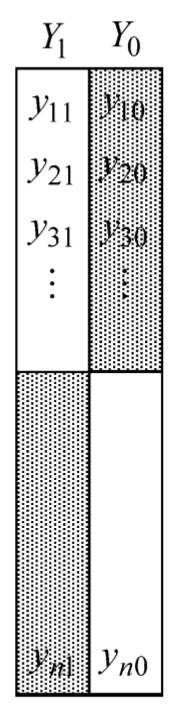
\includegraphics[height=2in]{img/potential_outcomes.png}
\end{figure}

\end{columns}

\end{frame}

%%%%%%%%%%%%%%%%%%%%%%%%%%%%%%%%%%%%%%%%%%%%%%%%%%%%%%%%%%%%%%%%%%%%%%%%%%%%%%%%
\begin{frame}{Na{\"i}ve comparison: $\EE [Y \vert D = 1] - \EE [Y \vert D=0]$}


Let's consider the averages of $Y_{1i}$, $Y_{0i}$, and $Y_i$:
\begin{align*}
\EE [ Y \vert D = 1 ] =& \EE [Y_0 + (Y_1 - Y_0) D \vert D = 1]
&&\because Y = Y_0 + (Y_1 - Y_0) D \\
=& \alert<2>{\EE[Y_1 \vert D = 1]}\\
\EE[Y \vert D = 0] 
% =& E [Y_0 + (Y_1 - Y_0) D \vert D = 0] \\
=& \alert<2>{\EE[Y_0 \vert D = 0]}
\end{align*}

\vspace{2ex}

We can re-write the observed difference in health outcomes as:
\begin{align*}
\EE [Y \vert D = 1] - \EE [Y \vert D=0] 
\onslide<2->{=& \alert<2>{\EE [Y_1 \vert D=1]} - \alert<2>{\EE [Y_0 \vert D=0]} \\}
\onslide<3->{=& \EE [Y_1 \vert D=1] \alert<3>{- \EE [Y_0 \vert D = 1] + \EE [Y_0 \vert D = 1]}  - \EE [Y_0 \vert D=0] \\}
\onslide<4->{=& \underbrace<5->{\EE [Y_1 - Y_0 \vert D = 1]}_{\text{Avg. treatment effect on treated}} 
\onslide<4->{+} \underbrace<5->{\EE [Y_0 \vert D = 1] - \EE [Y_0 \vert D=0]}_{\text{Selection bias}}}
\end{align*}

\end{frame}

%%%%%%%%%%%%%%%%%%%%%%%%%%%%%%%%%%%%%%%%%%%%%%%%%%%%%%%%%%%%%%%%%%%%%%%%%%%%%%%%
\begin{frame}{Na{\"i}ve comparison (cont.)}

Observed difference in earnings equals the average treatment effect (ATE) on the treated plus selection bias:
\begin{align*}
\EE [Y \vert D = 1] - \EE [Y \vert D=0] 
% =& \EE [Y_1 \vert D=1] { - \EE [Y_0 \vert D = 1] + \EE [Y_0 \vert D = 1]}  - \EE [Y_0 \vert D=0] \\
=& \underbrace{\EE [Y_1 - Y_0 \vert D = 1]}_{\text{ATE on treated}} 
+ \underbrace{\EE [Y_0 \vert D = 1] - \EE [Y_0 \vert D=0]}_{\text{Selection bias}}
\end{align*}
ATE on treated is the average causal effect of college attendance on those who went to college:
\begin{equation*}
    \EE [Y_1 \vert D=1] - \EE [Y_0 \vert D = 1] = \EE [Y_1 - Y_0 \vert D = 1]
\end{equation*}
Selection bias:
\begin{equation*}
    \EE [Y_0 \vert D = 1] - \EE [Y_0 \vert D=0]
\end{equation*}
\textbf{What do you think selection bias looks like in this example?}

\pause
\begin{itemize}
    \item The difference in $Y_{0i}$ between those who went to college and those who didn't 
    \item Consider someone who went to college. Now assume that person didn't go. Their expected earnings may be higher than those of someone who didn't go to college at all 
    \begin{itemize}
        \item[$\implies$] Those who didn't go to college, on average, have lower values of $Y_{0i}$

        \item[$\implies$] Selection bias is positive
    \end{itemize}
\end{itemize}
\end{frame}

%%%%%%%%%%%%%%%%%%%%%%%%%%%%%%%%%%%%%%%%%%%%%%%%%%%%%%%%%%%%%%%%%%%%%%%%%%%%%%%%
\begin{frame}{Random assignment and selection bias}

Random assignment ($Y_0, Y_1 \perp D$) will solve the selection problem
\begin{itemize}
    \item Causes selection bias to equal zero
\end{itemize}
\begin{align*}
    \EE [Y_1 \vert D = 1] = \EE[Y_1 \vert D = 0] = \EE [Y_1] \quad
    \text{and}& \quad \EE [Y_0 \vert D = 0] = \EE [Y_0 \vert D = 1] = \EE [Y_0] \\
    \implies&
    \EE [Y_0 \vert D = 1] - \EE [Y_0 \vert D = 0] = 0 \\
    \implies&
    \text{Selection bias is 0} \\
    \implies&
    \text{Na{\"i}ve comparison = ATE on treated}
\end{align*}
What do we do when we don't have random assignment?

\end{frame}

%%%%%%%%%%%%%%%%%%%%%%%%%%%%%%%%%%%%%%%%%%%%%%%%%%%%%%%%%%%%%%%%%%%%%%%%%%%%%%%%
\begin{frame}{Conditional Independence Assumption}

Independence of potential outcomes and the treatment:
\begin{itemize}
     \item [$\implies$] ($Y_0, Y_1 \perp D$)
     \item [$\implies$] randomization
\end{itemize} 
What happens when we don't have independence? Meaning the occurrence of $D$ influences the occurrence of $Y_0$ and $Y_1$ (or vice versa)?

\vspace{3ex}
Perhaps we can condition on certain variables $X$, such that the treatment $D_i$ and the potential outcomes $Y_{1i}, Y_{0i}$ LOOK independent
\begin{equation*}
    \{Y_{0i}, Y_{1i}\} \perp D_i \vert X_i
\end{equation*}

\vspace{3ex}

\end{frame}

%%%%%%%%%%%%%%%%%%%%%%%%%%%%%%%%%%%%%%%%%%%%%%%%%%%%%%%%%%%%%%%%%%%%%%%%%%%%%%%%
\begin{frame}{Conditional independence}

Conditional independence assumption: 
\begin{equation*}
    \{Y_{0i}, Y_{1i}\} \perp D_i \vert X_i
\end{equation*}
Intuitively: occurrence of $D_i$ does not influence the occurrence of $Y_{0i}$ or $Y_{1i}$, or vice versa, conditional on knowing $X_i$:
\begin{align*}
    \EE[Y_{0i} \vert D_i, X_i] &= \EE [Y_{0i} \vert X_i] \\
    \EE[Y_{1i} \vert D_i, X_i] &= \EE [Y_{1i} \vert X_i] 
\end{align*}

\begin{columns}
\column{0.4\linewidth}
\begin{figure}
\begin{tikzpicture}
\node [draw, circle] (D) {D};
\node [draw, circle, below =of D] (Y) {Y};
\node [draw, circle, right =of D] (X) {X};
\draw (D) edge[->] (Y);
\draw (X) edge[->] (D);
\draw (X) edge[->] (Y);
\end{tikzpicture}
\end{figure}

\column{0.6\linewidth}
\begin{figure}
\begin{tikzpicture}
\node [draw] (D) {College attendance};
\node [draw, below =of D] (Y) {Earnings};
\node [draw, right =of D] (X) {Ability};
\draw (D) edge[->] (Y);
\draw (X) edge[->] (D);
\draw (X) edge[->] (Y);
\end{tikzpicture}
\end{figure}

\end{columns}

\end{frame}


%%%%%%%%%%%%%%%%%%%%%%%%%%%%%%%%%%%%%%%%%%%%%%%%%%%%%%%%%%%%%%%%%%%%%%%%%%%%%%%%
\begin{frame}{Selection bias under CIA}

Under conditional independence assumption, selection bias disappears conditional on $X_i$:
\begin{align*}
    \EE [Y_{0i} \vert X_i, D_i = 1] - \EE [Y_{0i} \vert X_i, D_i = 0]
    =& \EE [Y_{0i} \vert X_i, D_i = 0] - \EE [Y_{0i} \vert X_i, D_i = 0] \\
    =& 0
\end{align*}
So we can write the difference in observed outcomes \textbf{conditional on $X_i$} as:
\begin{align*}
    \EE [Y_i \vert X_i, D_i = 1] - \EE [Y_i \vert X_i, D_i = 0] 
    &= \EE [Y_{1i} \vert X_i, D_i = 1] - \EE [Y_{0i} \vert X_i, D_i = 0] \\
    &= \EE [Y_{1i} \vert X_i] - \EE [Y_{0i} \vert X_i] \\
    &= \EE [Y_{1i} - Y_{0i} \vert X_i]
\end{align*}
Given the CIA, comparisons of average earnings (conditional on $X_i$) have a causal interpretation
\end{frame}

%%%%%%%%%%%%%%%%%%%%%%%%%%%%%%%%%%%%%%%%%%%%%%%%%%%%%%%%%%%%%%%%%%%%%%%%%
%%%%%%%%%%%%%%%%%%%%%%%%%%%%%%%%%%%%%%%%%%%%%%%%%%%%%%%%%%%%%%%%%%%%%%%%%%%%%%%%
\begin{frame}{When treatment takes on more than two values}

Expanding CIA assumption to relations that can take on more than two values, such as when $s_i = \{0, 1, \dots, 16\}$ equals years of schooling:
\begin{equation*}
    Y_{si} = f_i (s)
\end{equation*}
Individual specific function:
\begin{itemize}
    \item Potential earnings that person $i$ would receive after obtaining $s$ years of education
    \item What would $i$ learn for any value of schooling
\end{itemize}

\vspace{2ex}
If $s$ could only take on two values, $s=12$ and $s=16$, then we're considering the value of college vs. no college:
\begin{equation*}
    Y_{0i} = f_i(12), \quad \quad Y_{1i} = f_i(16)
\end{equation*}

\end{frame}

%%%%%%%%%%%%%%%%%%%%%%%%%%%%%%%%%%%%%%%%%%%%%%%%%%%%%%%%%%%%%%%%%%%%%%%%%%%%%%%%
\begin{frame}{CIA with non-binary treatment}

CIA in this more general set-up:
\begin{equation*}
    Y_{si} \perp s_i \vert X_i, \quad \forall s_i
\end{equation*}
\begin{itemize}
    \item In randomized experiments (RCTs), $s_i$ is randomly assigned based on covariates $X_i$
    \item In observational studies, the CIA means $s_i$ is \textbf{as good as randomly assigned} conditional on $X_i$
\end{itemize}
Under conditional independence assumption, comparisons of average earnings across schooling levels have a causal interpretation:
\begin{equation*}
    \EE [Y_i \vert X_i, s_i = s] - \EE[Y_i \vert X_i, s_i = s - 1] = \EE [f_i(s) - f_i(s - 1) \vert X_i]
\end{equation*}
For example, average causal effect of high school graduation:
\begin{align*}
    \EE [Y_i \vert X_i, s_i = 12] - \EE[Y_i \vert X_i, s_i = 11] =& \EE [f_i (12) \vert X_i, s_i = 12] - \EE [f_i (11) \vert X_i, s_i = 11] \\
    =& \EE [f_i(12) - f_i(11) \vert X_i, s_i = 12] 
\end{align*}
\begin{itemize}
    \item Here, selection bias would come from the differences in potential earnings of high school graduates and non-graduates
    \item Under CIA, high school graduation is independent of potential earnings conditional on $X_i$, so selection bias disappears
\end{itemize}

\end{frame}

%%%%%%%%%%%%%%%%%%%%%%%%%%%%%%%%%%%%%%%%%%%%%%%%%%%%%%%%%%%%%%%%%%%%%%%%%%%%%%%%
\begin{frame}{CIA and regression}

Regression is an empirical strategy that turns CIA into causal effects:
\begin{itemize}
    \item Assume $f_i(s)$ is linear in $s$, and the same for everyone, except for an additive term $\eta_i$:
    \begin{equation*}
        f_i(s) = \alpha + \rho s + \eta_i
    \end{equation*}
    \item \textbf{Linear constant effects model}: equation is linear, and the functional relationship is the same for everyone
    \item Only individual-specific part of $f_i(s)$ is mean-zero $\eta_i$, which captures unobserved factors that determine potential earnings
\end{itemize}
Observed value will be:
\begin{equation*}
    Y_i = \alpha + \rho s_i + \eta_i, 
\end{equation*}
Note that $s_i$ is correlated with $\eta_i$: $\EE [\eta_i \vert s_i] \neq 0$. If we ran this regression, we'd expect selection bias to impact our results.

\end{frame}

%%%%%%%%%%%%%%%%%%%%%%%%%%%%%%%%%%%%%%%%%%%%%%%%%%%%%%%%%%%%%%%%%%%%%%%%%%%%%%%%
\begin{frame}{CIA and regression (cont.)}

Assume CIA holds, and $\eta_i$ has the form:
\begin{equation*}
    \eta_i = X_i^\prime \gamma + v_i
\end{equation*}
where: 
\begin{itemize}
    \item $\gamma$ is a vector of population regression coefficients that satisfies $\EE [\eta_i \vert X_i] = X_i^\prime \gamma$
    \item $v_i$ and $X_i$ are uncorrelated by construction
\end{itemize}
Then, because of the CIA:
\begin{align*}
    \EE [f_i(s) \vert X_i, s_i] &= \EE[f_i (s) \vert X_i] \\
    &= \alpha + \rho s + \EE [\eta_i \vert X] \\
    &= \alpha + \rho s + X_i^\prime \gamma
\end{align*}
The residual in the linear causal model $v_i$ is uncorrelated with $s_i$ and $X_i$, and $\rho$ is the causal effect of interest:
\begin{equation*}
    Y_i = \alpha + \rho s_i + X_i^\prime + v_i
\end{equation*}

\end{frame}



\end{document}